\subsection{Manuscript Management}
\subsubsection{Creating a Manuscript}
\textbf{Using the Wizard}\\
	Creating a manuscript (e.g. book, letter, poem, etc.), is a very easy process. The manuscript you've created will be available to you immediately after creation. At which point you may edit it as you wish. Let us have a look at the steps necessary to creating your masterpiece.\\ \\

	\begin{itemize}
		\item Assuming that logging in has been successfully achieved, the location should be the homepage of Figbook. Click on "Catalogue" on the top-leftmost block on the blocks on the screen. You should now see this page:
		
		\begin{figure}[h]
		\centering
			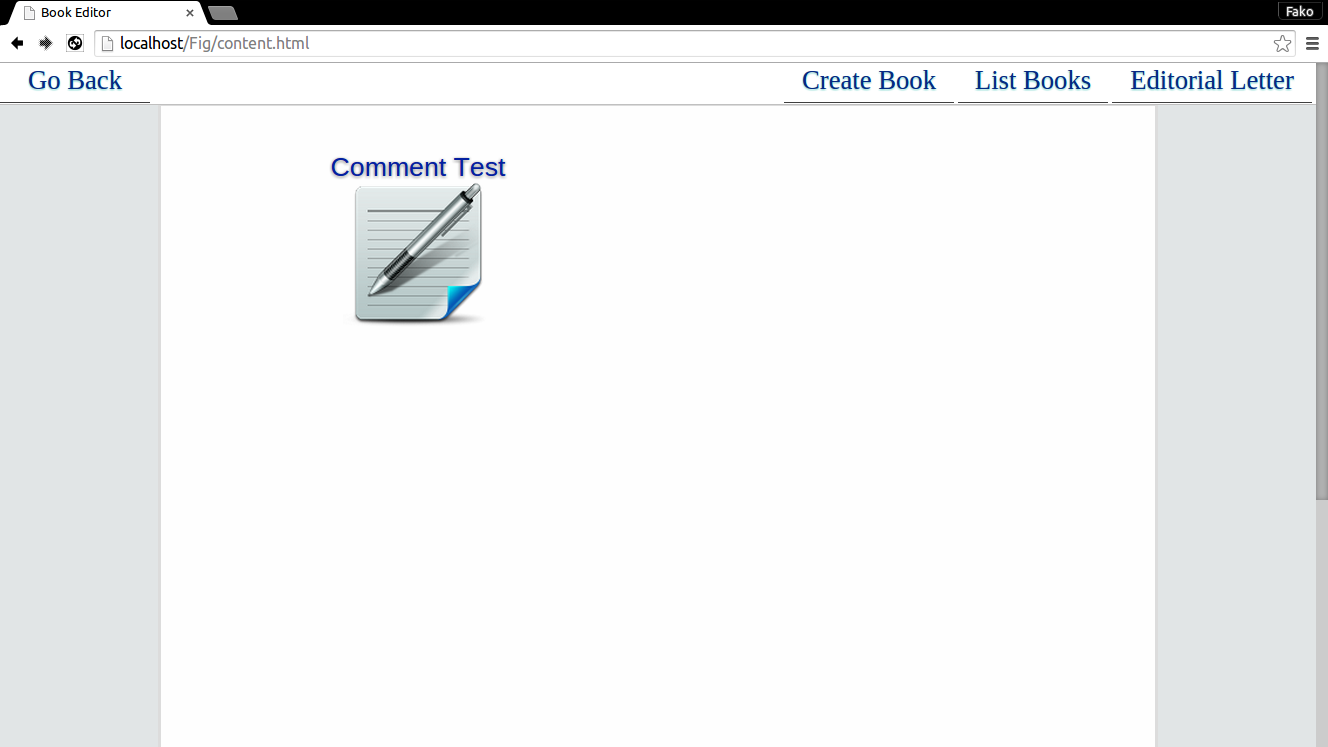
\includegraphics[scale=0.3]{images/SeePage.png}
			\caption{Create Manuscript button}
		\end{figure}
		
		Click 'Create Manuscript' to open the wizard.
		\item The book title, author name and author surname should be entered. Click next when done, or back to return to the previous page.
		
		\begin{figure}[h]
			\centering
			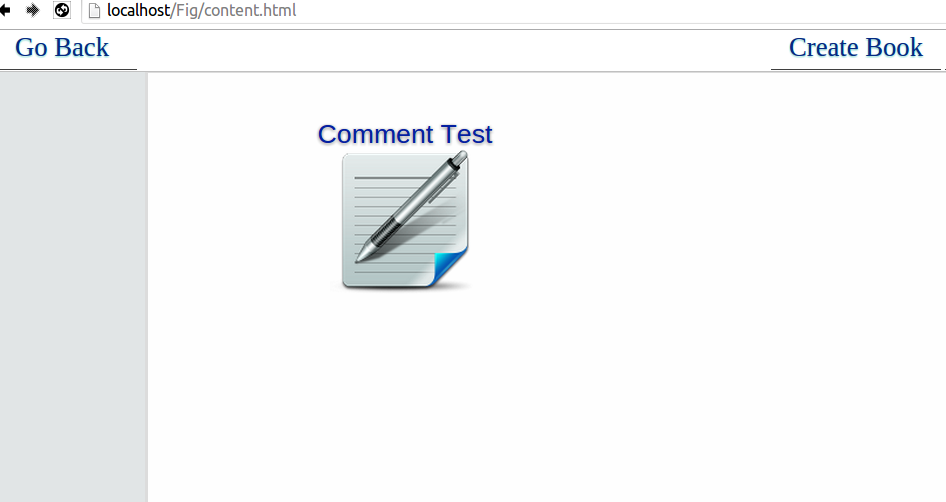
\includegraphics[scale=0.5]{images/SelectBook2.png}
			\caption{After creating a book, you will be taken back to the list of books.}
		\end{figure}
		\newpage
		\item A preface on the content of the book should be entered. It clear and decriptive to optimize the quality of the selected piece of literature (Note that this is not compulsory. You may leave it blank). 
		
		\begin{figure}[h]
		\centering
			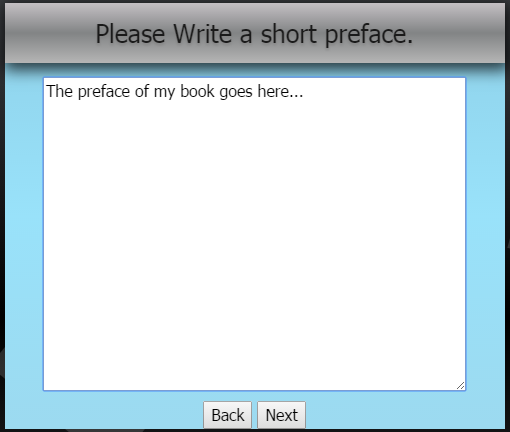
\includegraphics[scale=0.5]{images/preface.png}
			\caption{Entering preface of the book}
		\end{figure}
	
		\item Clicking next will create your manuscript and return you to your list of books. Your manuscript will be listed there. You can click on it to start editing.
		\end{itemize}
\subsubsection{Editing a Manuscript}
	Editing a manuscript entails loading the content of an existing manuscript into an open text area for the author to edit. 

	\begin{itemize}
		\item To access all the manuscripts available to you, from the home page click on the 'Catalogue' button. This should populate the page with all the manuscripts available to the user. 
		\begin{figure}[h]
			\centering
			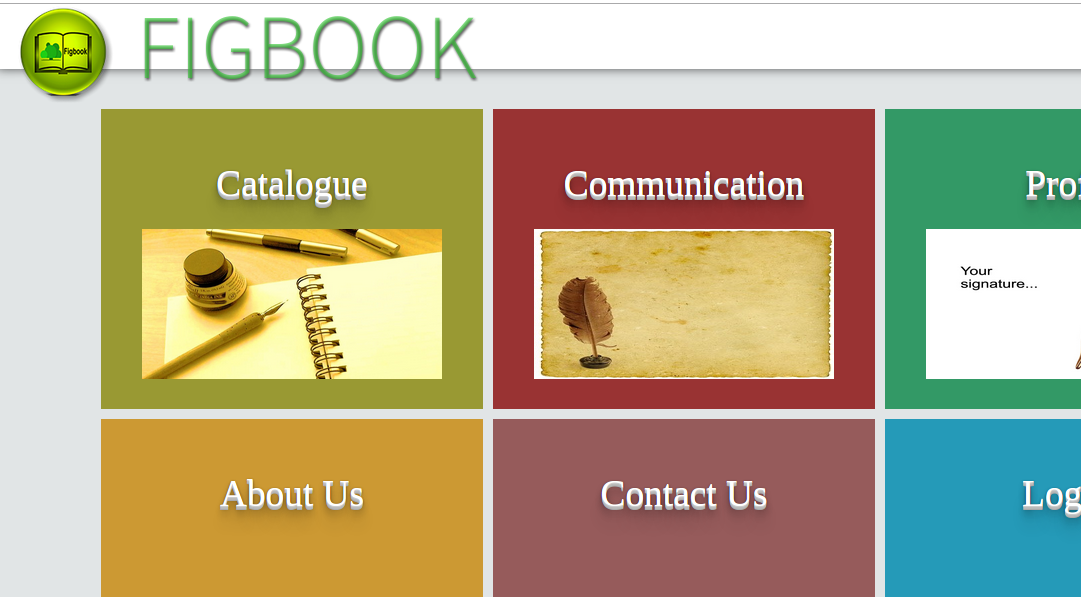
\includegraphics[scale=0.3]{images/SelectBook.png}
			\caption{catalogue button on home page}
		\end{figure} 
		
		\newpage
		\item Open a manuscript by clicking on it. This should take you to the document layout of the manuscript of interest. Click on any section you want to edit and a text editor will open for editing. In the figure below, clicking anywhere on the Preface will open a text editor for the user to edit the preface.
		\begin{figure}[h]
			\centering
			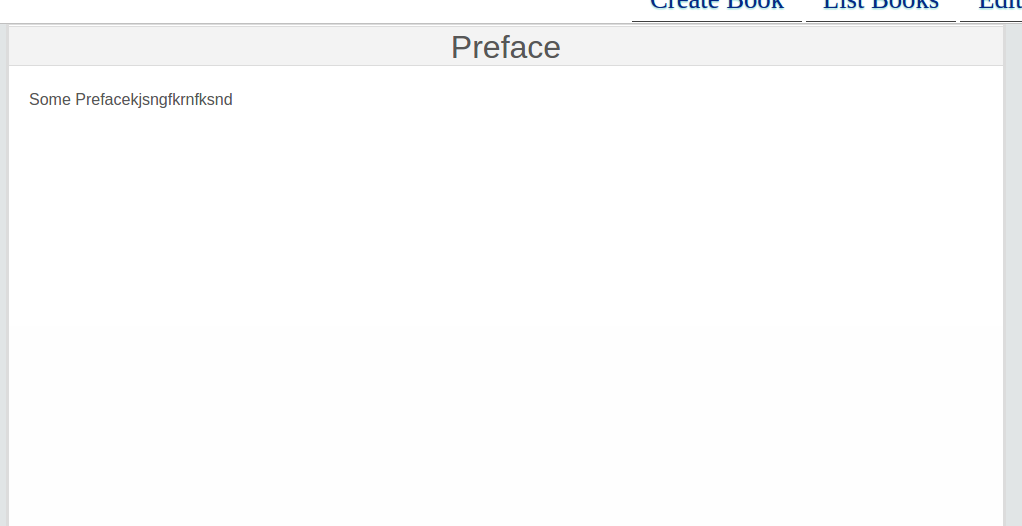
\includegraphics[scale=0.3]{images/EditSection.png}
			\caption{Edit a section by clicking on it}
		\end{figure} 
		\item you may edit any area of the section and click the 'Save' button when you wish to save the changes made. This should take you back to the document view of the manuscript.
		
		\begin{figure}[h]
			\centering
			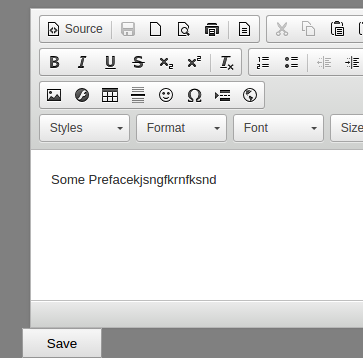
\includegraphics[scale=0.5]{images/SaveChanges.png}
			\caption{save section button}
		\end{figure} 
	\end{itemize}
	
\subsubsection{Commenting on a Manuscript}
Manuscript comments are there to provide side-notes to the author about the manuscript being written. Comments belong to specified sections of the manuscript and can be added by use of a simple procedure.

\begin{itemize}
	\item By expanding the arrow that appears on the left-hand side of your manuscript, a comment box should appear as shown below.
	
	\begin{figure}[h]
			\centering
			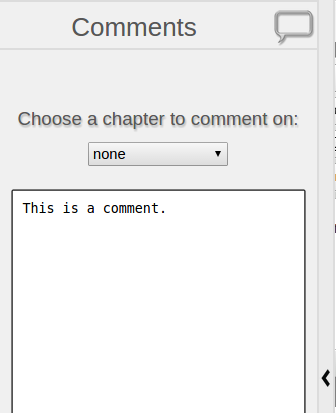
\includegraphics[scale=0.6]{images/SectionComment.png}
			\caption{Section Comment box.}
		\end{figure} 
		
	\item Use the drop-down list to select the particular section of the manuscript on which you want to comment.
	\item Enter a comment in the comment edit box below the drop-down list.
	\item Use the Comment 'Save' button to Save the comment. 	
	
	\begin{figure}[h]
			\centering
			
\includegraphics[scale=0.6]{images/CommentSaveButton.png}
			\caption{Save a comment.}
		\end{figure} 
\end{itemize}

\newpage
\subsubsection{Include an Editorial Letter}
Editorial Letters can be made on manuscripts By Expanding the arrow that appears on the right-hand side of the manuscript or by clicking on the 'Editorial Letter' link above on the window. Upon expansion of the editorial letter, this is what you should see.

\begin{figure}[h]
			\centering
			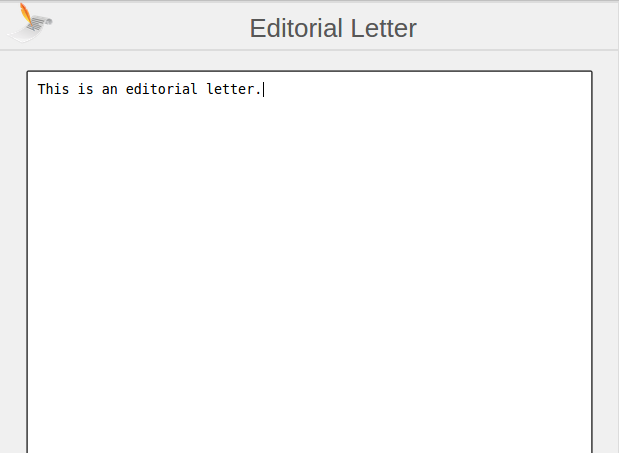
\includegraphics[scale=0.6]{images/EditorialLetter.png}
			\caption{Editorial Letter Box.}
		\end{figure} 
		
		\begin{itemize}
			\item Simple enter the contents of the letter.
			\item The Letter is linked to the entire manuscript and not just a section being worked on.
			\item Use the 'Send' button to save the changes to your editorial letter and to link it to the manuscript in question.
			
			\begin{figure}[h]
			\centering
			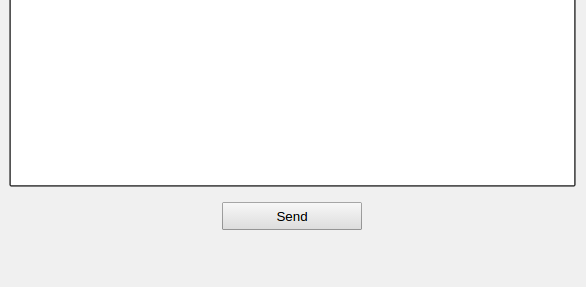
\includegraphics[scale=0.4]{images/SendEditorialLetter.png}
			\caption{Editorial Save Button.}
		\end{figure}  
		\end{itemize}